\begin{appendices}
\chapter{Self-appraisal}
The following appendix offers discussion related to the project process in the form of a critical self-evaluation, a personal reflection paired with lessons learnt, and thorough discussion on the legal, social, ethical, and professional issues related to the project.

\section{Critical self-evaluation}
Given the achievements of the project and my personal development I am pleased with how the process has gone. I achieved each goal set out at the beginning of the project, met the overall project aim, and built a high-quality solution. Regardless of this, there are several areas to consider in terms of improvement. Reviewing the entire project process reveals what went well and what could be improved upon.

After presenting several project ideas to my supervisor in early October, we selected a project idea within the intersection of our interests: SR (as suggested by my supervisor) in remote sensing (as suggested by myself). Finding an initial idea that fits in this intersection meant we were both enthusiastic about the project, leading to a greater interest, better communication, and a greater motivation to learn. 

Following the initial idea was a lengthy period of background research. My findings showed that the general research direction in the field of SR was deep learning, more specifically GANs. Being completely new to the field, much of my background research was spent upskilling in deep learning, delving into topics such as neural networks, gradient descent, optimisation, datasets, regularisation, CNNs, and eventually GANs. Spending such a significant amount of time in this upskilling phase was invaluable to producing a good result, as many of the topics are complex, especially as they were entirely new to me at the time. The main downside of spending so much time upskilling in deep learning, was that I spent very little time actually planning the project or researching a variety of SR solutions, which will have cost me report writing time in the long run. Regardless, the extensive time spent upskilling was vital to the project success.

Following this upskilling phase was the submission of my project idea and scope. Given the upskilling period, I was confident filling this in, and the initial idea is very much in line with the final project outcome. The summary provided for this submission was the foundation of the project introduction, and kept me focused on the primary goal. The only part of the project scope that was not a success was the timeline plan. Given the rest of my commitments at university I did not manage to spend nearly as much time as I had hoped on the project in semester one, which put me behind when beginning development in semester two.

After the submission of the project scope and outline no significant work was completed on the project until after the winter exam period, given my extensive commitments. Following the exam period, I spent significantly more time on the project due to a decrease in other commitments. The initial phase was spent reviewing my learnings from semester one, which was a fast process as much of the legwork was completed before then. This meant that I could begin my project with haste and not waste time with upskilling, again showing how crucial the upskilling period was.

The beginning of the process was to practise implementing GANs in Keras. As GAN models are complex they require a customised training sequence, which is not entirely intuitive without reviewing the Keras documentation. As a result, I spent a good amount of time implementing a conditional GAN, and an unconditional GAN based on the Keras documentation. This allowed me to put my previous theoretical learnings into practice, reinforcing what I had learnt whilst also overcoming some difficulties related to implementing a GAN in Keras for the first time. The aim of this was to be equipped to implement SRGAN, which was the model I had selected to implement and improve, as described in Chapter 2.

Following implementation practise, the results of which can be found in the project repository, was exploring the different datasets we could use prior to implementing SRGAN.\@ Doing this allowed me to move closer to the real implementation, as I would have had lots of domain knowledge, implementation practise, and access to an appropriate dataset. The dataset was selected based on a review of commonly used remote sensing datasets. Before systematically testing memory constraints to decide a final dataset size, a default size of 2048 was selected whilst we were implementing, which was beneficial as it allowed me to focus on the implementation fully and not become distracted by the dataset.

Following this, I was well-equipped to implement SRGAN.\@ Due to the iterative learning process I introduced, the SRGAN implementation was fairly quick and painless. In the few moments where I was unsure or stuck I referenced an online implementation for rough guidance, but ensured I did not rely on it. This online implementation is properly credited in the following appendix.

Following this, I spent time enabling GPU training on the university machines, along with SSH access. This let me train the models significantly faster, which resulted in me producing the first set of good SR reconstructions, which ended up motivating me as a significant milestone in the project. I initially encountered an issue with the reconstructions where the colours were seemingly random, but the image structure was intact. After investigation, I discovered it was due to me not taking due care to fully read the implementation details offered by the SRGAN paper, as I had missed the pretraining of the SRGAN generator, along with the image patches. Discovering this was useful not only for the project, but also for me personally as it showed me that I needed to take extra care reviewing subjects in the project.

Following the initial success of the project came the most difficult period. At this point I was experiencing uncertainty with the direction of the project as a whole. I had technically achieved the project aim already at this point, however there was much room for improvement. This is where I spent time reviewing more recent solutions and taking a more detailed look at SRGAN as a whole. This was also difficult as it meant I was unable to begin my report section as I was unsure how much my original ideas would change. After careful consideration, I eventually decided on attempting to improve the SRGAN loss function through the method explained in the project. This phase of the project was unexpected at the beginning and was not included in my initial project plan, which was an oversight on my part. Even though it was a difficult process, I believe it was necessary for the suggestion of a well considered and high-quality improvement to SRGAN.\@

At this point, I followed the implementation of the losses and the training parameters as outlined in Chapter 3. I spent a significant amount of time training the final models and evaluated them using the appropriate loss metrics. During this implementation time I had begun writing my final report. The point at which I began writing was not ideal and left me with less time than desired, but was symptomatic of the difficulties I encountered with project direction. Following the completion the implementation, training and testing, the remaining time was spent writing and iteratively refining my report.

Overall, I am pleased with the final result. I have exerted a massive amount of effort in terms of upskilling, research, implementation, training, testing, etc.\ to produce a solution that is of a high standard. The project process was not without its flaws and resulted in less time than desired for the report writing portion, but the time was spent ensuring the quality of the solution which I believe reflects in the final result.

\section{Personal reflection and lessons learned}
Completing this project marked a significant period of personal development for me. It was without a doubt the most technically and theoretically demanding piece of work I have completed, whilst also being the longest persisting project I have taken on.

The nature of the project required me to gain a level of knowledge on an academic subject that I had not possessed before. Failure to gain the necessary knowledge would mean failure to implement a proper solution, and therefore I would not achieve the main project aim. To ensure that I did in fact meet the project aim, I invested significant time into the SR reconstruction problem, the theory of deep learning, implementing neural networks, datasets, how to train a model, acceptable evaluation tests etc. The result is a high level of knowledge on a complex academic subject, and a high-quality solution that represents this level of knowledge.

Regardless of this, there are still areas I can identify as personal shortcomings in the project. In a general sense I did not spend nearly enough time planning, which resulted in delays related to project direction, leading to less time to complete other necessary project components. Additionally, I could have improved my communication with my supervisor throughout the project, but especially in the planning phase. The periods that I did plan were fast and painless, but the ones that I did not cost time, were difficult to navigate, and harmed my motivation. Liaising with my supervisor more frequently would have resulted in faster resolutions to my issues and a stronger project overall. This is not to say I did not communicate with my supervisor at all, I attended every meeting and asked for help were absolutely necessary, but I could have received more help in some difficult areas.

Through this process I have learned a number of lessons relating to conducting a project of this size, about the academic process, and about myself. Firstly, I learned that planning is absolutely essential when completing a project of this size. Whilst seemingly cumbersome at first, planning absolutely saves time in the long run. I have also learned that it is important to plan for unforeseen circumstances. Whilst foresight is not possible, allocating some amount of time for unexpected setbacks and issues gives the timeline some leeway, and derailment of the project plan is unlikely. I have also learnt a great deal about the academic process, not only from executing it myself, but also from exposing myself to published literature. Systematically reading and evaluating literature exploring the boundary of human knowledge enforced a newfound respect for the process required to create such a publication, whilst also instilling such behaviours in myself. I have learnt how to reason about complicated topics and form opinions for myself based on objective evidence, which is a skill I will utilise significantly more in the future. Finally, I have learnt more about my process and ability than I ever have before. I know how to respect my process, whilst also knowing when to enforce discipline in times of difficulty. This project, with its successes and failures, has provided me an opportunity to learn and develop at a level of academic complexity that I may not experience again, which I am incredibly grateful for.

\section{Legal, social, ethical and professional issues}
The following section covers the legal, social, ethical, and professional issues related to the project, and how we accounted for each.

\subsection{Legal issues}
Publicly available datasets used to train our solutions are distributed with licences. These licences specifically describe the usage rights for the dataset, and failing to comply breaks intellectual property law, which could result in legal action. Before using any datasets, we reviewed the usage licences to ensure we were not breaking any laws by using them.

Another legal issue, albeit very unlikely, is related to the fact that we are technically generating imagery that does not exist. Our solutions are producing HR estimations of LR imagery, which means it will never perfectly recreate the image. As such, it is important to consider that there may be a scenario where our solution could produce an image of a scene that suggests a negative context relating to an individual or organisation. If this turns out to be false, then we may be breaking defamation laws. In reality, it is incredibly unlikely that we generate a scene that suggests nefarious activities. Nonetheless, it is interesting to highlight.

\subsection{Social issues}
The primary social issue to consider is global climate change. Remote sensing imagery is intrinsically linked to climate change through its common use in the field. We must consider that our solution could be used to spread misinformation about climate change in the form of inaccuracies produced by our estimation, e.g.\ our SR reconstruction may show more of a reduction in forest cover than is true. Whilst important to consider, it is incredibly unlikely that our solution will be used for these purposes, and so is not a reason to change our focus.

\subsection{Ethical issues}
As we used a pre-existing solution as the foundation of ours, it was important to correctly credit the original creators. Failure to do so could be considered plagiarism, which would nullify the project. At every stage of the project we cite the literature we collected our understanding from, whilst crediting each section of the implementation that was not from us directly. Any external materials we used to help us are also included in the following appendix.

Another ethical issue is related to the NWPU-RESISC45 dataset, which is composed of remote sensing imagery. Remote sensing imagery poses ethical concerns as it provides information about massive areas of space without the explicit consent from the people it may capture. Remote sensing imagery with high-spatial resolution can reveal private information about an individual or organisation, based on the movement of their possessions (cars, infrastructure, resources). As a result it is important to consider whether it is ethical to use remote sensing imagery for this project. Prior to capturing remote sensing imagery, special permission has to be granted by the relevant governments. This barrier restricts who can capture remote sensing imagery. We can assume that the individuals that the imagery may affect have (usually) democratically elected their government, and as a result the government acts on their behalf. If we assume this, then any remote sensing imagery capture that a government approves is also approved on behalf of their citizens. This observation suggests that using remote sensing imagery is ethically compliant.

\subsection{Professional issues}
Not conducting ourselves professionally would cause the project itself to not appear professional. We ensured an excellent level of professionalism throughout the project. We consistently liaised professionally with our project supervisor to maintain a respectful environment. We ensured that we followed professional programming practices in the form of modular, reusable code. The project report uses professional language, leading to quality in the final result.

\chapter{External Material}\label{app:external_material}
This project uses material from various external source to aid in the implementation and testing of our solutions. All external material used is presented here.

\section{\code{Python} libraries}
The following is the full list of \code{Python} libraries used for the development of this project.
\begin{itemize}
    \item \code{Keras}
    \item \code{TensorFlow}
    \item \code{NumPy}
    \item \code{TensorFlow Datasets}
    \item \code{OpenCV--Python}
    \item \code{scikit--image}
    \item \code{scikit--learn}
    \item \code{matplotlib}
    \item \code{glob}
    \item \code{Pandas}
\end{itemize}

\section{NWPU-RESISC45 dataset}
The NWPU-RESISC45 dataset was accessed and loaded through the \code{TensorFlow Datasets} library. The dataset must be manually placed in the correct repository in the \code{TensorFlow Datasets} directory prior to using the data loader function. 

The dataset was downloaded from: \textcolor{blue}{https://1drv.ms/u/s!AmgKYzARBl5ca3HNaHIlzp\_IXjs}

\section{Set5 and Set14}
Set5 and Set14 are widely available online due to their widespread use. For this project, we used the public GitHub repository for the SelfExSR~\cite{selfexsr} model as the source for the datasets. The repository was cloned and the appropriate LR and HR pairs were extracted.

The repository can be found here: \textcolor{blue}{https://github.com/jbhuang0604/SelfExSR}

\section{SRGAN implementation}
Whilst implementing SRGAN from scratch we used an online implementation~\cite{srganImplementation} as a reference point to aid us when encountering issues: \textcolor{blue}{https://pyimg.co/lgnrx}

\section{Pretrained classifiers}
In this project we aimed to improve loss by using a variety of pretrained image classifiers. Each of the pretrained classifiers is available as a part of the \code{Keras} library. The full list is as follows:
\begin{table}[ht]
    \centering
    \resizebox{\textwidth}{!}{
        \begin{tabular}{llllllll}
            \toprule
            \textbf{Model} & \textbf{Size (MB)} & \textbf{Top-1 Accuracy} & \textbf{Top-5 Accuracy} & \textbf{Parameters} & \textbf{Depth} & \textbf{ms/step (CPU)} & \textbf{ms/step (GPU)} \\
            \midrule
            Xception & 88 & 79.00\% & 94.50\% & 22.9M & 81 & 109.4 & 8.1 \\ 
            VGG16 & 528 & 71.30\% & 90.10\% & 138.4M & 16 & 69.5 & 4.2 \\ 
            VGG19 & 549 & 71.30\% & 90.00\% & 143.7M & 19 & 84.8 & 4.4 \\ 
            ResNet50 & 98 & 74.90\% & 92.10\% & 25.6M & 107 & 58.2 & 4.6 \\ 
            ResNet50V2 & 98 & 76.00\% & 93.00\% & 25.6M & 103 & 45.6 & 4.4 \\ 
            ResNet101 & 171 & 76.40\% & 92.80\% & 44.7M & 209 & 89.6 & 5.2 \\ 
            ResNet101V2 & 171 & 77.20\% & 93.80\% & 44.7M & 205 & 72.7 & 5.4 \\ 
            ResNet152 & 232 & 76.60\% & 93.10\% & 60.4M & 311 & 127.4 & 6.5 \\ 
            ResNet152V2 & 232 & 78.00\% & 94.20\% & 60.4M & 307 & 107.5 & 6.6 \\ 
            InceptionV3 & 92 & 77.90\% & 93.70\% & 23.9M & 189 & 42.2 & 6.9 \\ 
            InceptionResNetV2 & 215 & 80.30\% & 95.30\% & 55.9M & 449 & 130.2 & 10 \\ 
            MobileNet & 16 & 70.40\% & 89.50\% & 4.3M & 55 & 22.6 & 3.4 \\ 
            MobileNetV2 & 14 & 71.30\% & 90.10\% & 3.5M & 105 & 25.9 & 3.8 \\ 
            DenseNet121 & 33 & 75.00\% & 92.30\% & 8.1M & 242 & 77.1 & 5.4 \\ 
            DenseNet169 & 57 & 76.20\% & 93.20\% & 14.3M & 338 & 96.4 & 6.3 \\ 
            DenseNet201 & 80 & 77.30\% & 93.60\% & 20.2M & 402 & 127.2 & 6.7 \\ 
            NASNetMobile & 23 & 74.40\% & 91.90\% & 5.3M & 389 & 27 & 6.7 \\ 
            NASNetLarge & 343 & 82.50\% & 96.00\% & 88.9M & 533 & 344.5 & 20 \\ 
            EfficientNetB0 & 29 & 77.10\% & 93.30\% & 5.3M & 132 & 46 & 4.9 \\ 
            EfficientNetB1 & 31 & 79.10\% & 94.40\% & 7.9M & 186 & 60.2 & 5.6 \\ 
            EfficientNetB2 & 36 & 80.10\% & 94.90\% & 9.2M & 186 & 80.8 & 6.5 \\ 
            EfficientNetB3 & 48 & 81.60\% & 95.70\% & 12.3M & 210 & 140 & 8.8 \\ 
            EfficientNetB4 & 75 & 82.90\% & 96.40\% & 19.5M & 258 & 308.3 & 15.1 \\ 
            EfficientNetB5 & 118 & 83.60\% & 96.70\% & 30.6M & 312 & 579.2 & 25.3 \\ 
            EfficientNetB6 & 166 & 84.00\% & 96.80\% & 43.3M & 360 & 958.1 & 40.4 \\ 
            EfficientNetB7 & 256 & 84.30\% & 97.00\% & 66.7M & 438 & 1578.9 & 61.6 \\ 
            EfficientNetV2B0 & 29 & 78.70\% & 94.30\% & 7.2M & ~ & ~ & ~ \\ 
            EfficientNetV2B1 & 34 & 79.80\% & 95.00\% & 8.2M & ~ & ~ & ~ \\ 
            EfficientNetV2B2 & 42 & 80.50\% & 95.10\% & 10.2M & ~ & ~ & ~ \\ 
            EfficientNetV2B3 & 59 & 82.00\% & 95.80\% & 14.5M & ~ & ~ & ~ \\ 
            EfficientNetV2S & 88 & 83.90\% & 96.70\% & 21.6M & ~ & ~ & ~ \\ 
            EfficientNetV2M & 220 & 85.30\% & 97.40\% & 54.4M & ~ & ~ & ~ \\ 
            EfficientNetV2L & 479 & 85.70\% & 97.50\% & 119.0M & ~ & ~ & ~ \\ 
            ConvNeXtTiny & 109.42 & 81.30\% & ~ & 28.6M & ~ & ~ & ~ \\ 
            ConvNeXtSmall & 192.29 & 82.30\% & ~ & 50.2M & ~ & ~ & ~ \\ 
            ConvNeXtBase & 338.58 & 85.30\% & ~ & 88.5M & ~ & ~ & ~ \\ 
            ConvNeXtLarge & 755.07 & 86.30\% & ~ & 197.7M & ~ & ~ & ~ \\ 
            ConvNeXtXLarge & 1310 & 86.70\% & ~ & 350.1M & ~ & ~ & ~ \\
            \bottomrule
        \end{tabular}
    }
    \caption{The full list of pretrained image classifiers available from \code{Keras}, complete with accuracy metrics.}
\end{table}

\chapter{Additional results}
This appendix lists the full performance results for the first and second passes of each model, measured with SSIM and PSNR.\@
\section{SSIM}
\begin{table}[h!]
    \centering
    \begin{tabular}{llll}
        \toprule
        \textbf{} & \textbf{Test set} & \textbf{Set5} & \textbf{Set14} \\
        \midrule
        \textbf{SRResNet} & \textbf{0.923512511} & \textbf{0.764288652} & \textbf{0.656266853} \\ 
        \textbf{SRGAN-VGG22-A} & 0.905764824 & 0.651937458 & 0.567257665 \\ 
        \textbf{SRGAN-VGG22-B} & 0.899406253 & 0.583057506 & 0.513103986 \\ 
        \textbf{SRGAN-VGG54-A} & 0.885763096 & 0.581977762 & 0.543001687 \\ 
        \textbf{SRGAN-VGG54-B} & 0.887826756 & 0.668649288 & 0.60303856 \\ 
        \textbf{SRGAN-Xception-A} & 0.88827486 & 0.594680597 & 0.551749692 \\ 
        \textbf{SRGAN-Xception-B} & 0.893502931 & 0.672196794 & 0.601761352 \\ 
        \textbf{SRGAN-ResNet152V2-A} & 0.897174099 & 0.604043834 & 0.553452834 \\ 
        \textbf{SRGAN-ResNet152V2-B} & 0.891586191 & 0.661280537 & 0.602065958 \\ 
        \textbf{SRGAN-InceptionV3-A} & 0.895036106 & 0.652690864 & 0.593326379 \\ 
        \textbf{SRGAN-InceptionV3-B} & 0.897317878 & 0.686002073 & 0.616420747 \\ 
        \textbf{SRGAN-InceptionResNetV2-A} & 0.897677893 & 0.64776438 & 0.587032919 \\ 
        \textbf{SRGAN-InceptionResNetV2-B} & 0.901842292 & 0.682449324 & 0.610296856 \\ 
        \textbf{SRGAN-MobileNetV2-A} & 0.880168377 & 0.646061649 & 0.586623268 \\ 
        \textbf{SRGAN-MobileNetV2-B} & 0.892767837 & 0.692512978 & 0.616935856 \\ 
        \textbf{SRGAN-DenseNet201-A} & 0.906292091 & 0.68875187 & 0.625844913 \\ 
        \textbf{SRGAN-DenseNet201-B} & 0.904457413 & 0.697771048 & 0.629857361 \\ 
        \textbf{SRGAN-NASNetLarge-A} & 0.890887913 & 0.631735007 & 0.575758199 \\ 
        \textbf{SRGAN-NASNetLarge-B} & 0.892950461 & 0.663674025 & 0.596643366 \\ 
        \textbf{SRGAN-EfficientNetV2L-A} & 0.894187301 & 0.545100159 & 0.506600485 \\ 
        \textbf{SRGAN-EfficientNetV2L-B} & 0.895758924 & 0.574972219 & 0.526297118 \\
        \bottomrule
    \end{tabular}
    \caption{The full list of SSIM results for SRResNet and both training passes of each SRGAN variation.}
\end{table}
\clearpage
\section{PSNR}
\begin{table}[h!]
    \centering
    \begin{tabular}{llll}
        \toprule
        \textbf{} & \textbf{Test set} & \textbf{Set5} & \textbf{Set14} \\
        \midrule
        \textbf{SRResNet} & \textbf{24.01698267} & 22.92709729 & 21.64800947 \\ 
        \textbf{SRGAN-VGG22-A} & 23.49328972 & \textbf{23.20232616} & \textbf{21.86280371} \\ 
        \textbf{SRGAN-VGG22-B} & 23.04977341 & 21.53465502 & 20.83574047 \\ 
        \textbf{SRGAN-VGG54-A} & 22.60240965 & 21.15867685 & 21.08800741 \\ 
        \textbf{SRGAN-VGG54-B} & 22.84813356 & 22.17587848 & 21.75984152 \\ 
        \textbf{SRGAN-Xception-A} & 22.83258858 & 21.21166409 & 20.90811321 \\ 
        \textbf{SRGAN-Xception-B} & 23.12606804 & 21.28395406 & 21.00604196 \\ 
        \textbf{SRGAN-ResNet152V2-A} & 23.10085499 & 21.04849148 & 21.00699857 \\ 
        \textbf{SRGAN-ResNet152V2-B} & 22.90267499 & 22.09173107 & 21.8309256 \\ 
        \textbf{SRGAN-InceptionV3-A} & 23.17347567 & 21.44583352 & 21.25388063 \\ 
        \textbf{SRGAN-InceptionV3-B} & 23.27200493 & 21.52440082 & 21.29319431 \\ 
        \textbf{SRGAN-InceptionResNetV2-A} & 23.30451732 & 21.88277315 & 21.07909838 \\ 
        \textbf{SRGAN-InceptionResNetV2-B} & 23.39098294 & 22.24528009 & 21.6065458 \\ 
        \textbf{SRGAN-MobileNetV2-A} & 21.78452233 & 21.08368593 & 20.58121556 \\ 
        \textbf{SRGAN-MobileNetV2-B} & 22.41608497 & 20.61076707 & 20.38898798 \\ 
        \textbf{SRGAN-DenseNet201-A} & 23.58496348 & 21.23221522 & 21.67087999 \\ 
        \textbf{SRGAN-DenseNet201-B} & 23.46598423 & 21.62907 & 21.78881868 \\ 
        \textbf{SRGAN-NASNetLarge-A} & 23.05990787 & 20.82933654 & 20.6679965 \\ 
        \textbf{SRGAN-NASNetLarge-B} & 23.02686718 & 20.86077465 & 20.96187622 \\ 
        \textbf{SRGAN-EfficientNetV2L-A} & 22.34285427 & 18.34391675 & 19.30080662 \\ 
        \textbf{SRGAN-EfficientNetV2L-B} & 22.53702017 & 19.64714065 & 20.00809338 \\
        \bottomrule
    \end{tabular}
    \caption{The full list of PSNR results for SRResNet and both training passes of each SRGAN variation.}
\end{table}

\chapter{Visualisations}
The following appendix offers some useful image visualisations of datasets and solution outputs.

\section{Model outputs}
\begin{figure}[H]
    \centering
    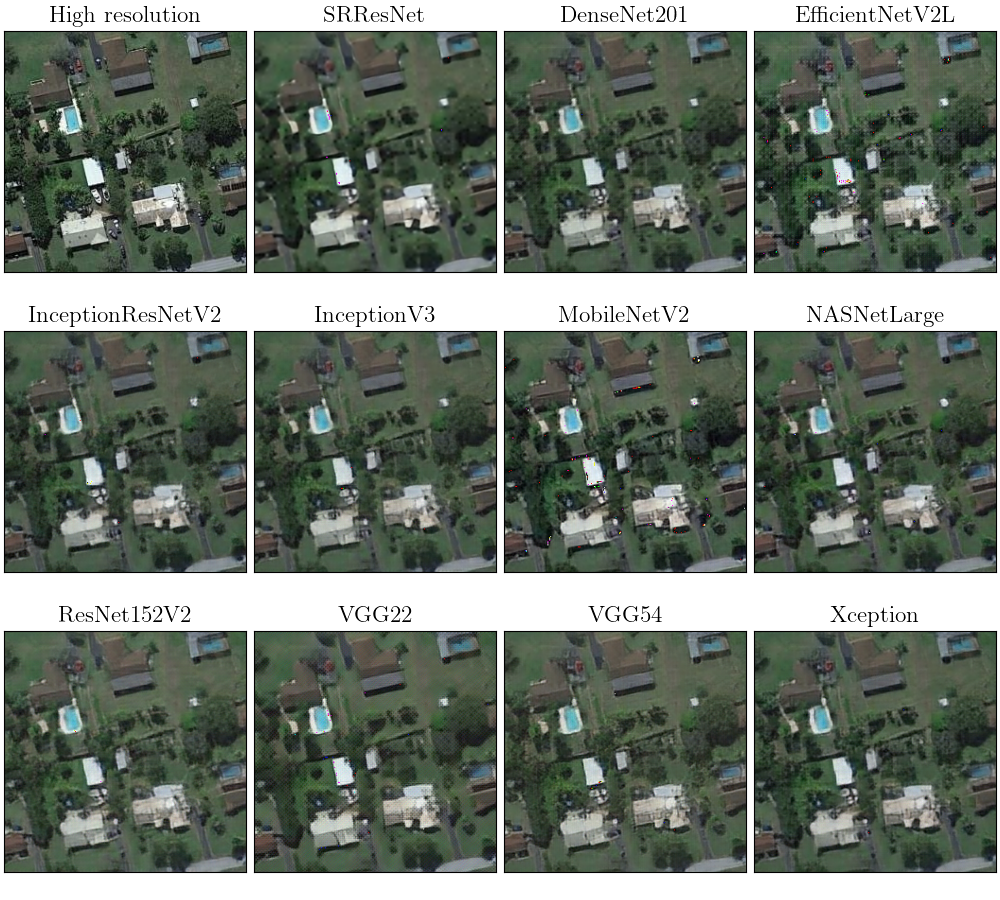
\includegraphics[width=\linewidth]{./assets/model_comparison.png}
    \caption{A comparison using a sample image from the NWPU-RESISC45 test set. The ground truth HR image, SRResNet, and SRGAN models with custom losses are shown.}\label{fig:model_comparison}
\end{figure}


\section{NWPU-RESISC45}
\begin{figure}[H]
    \centering
    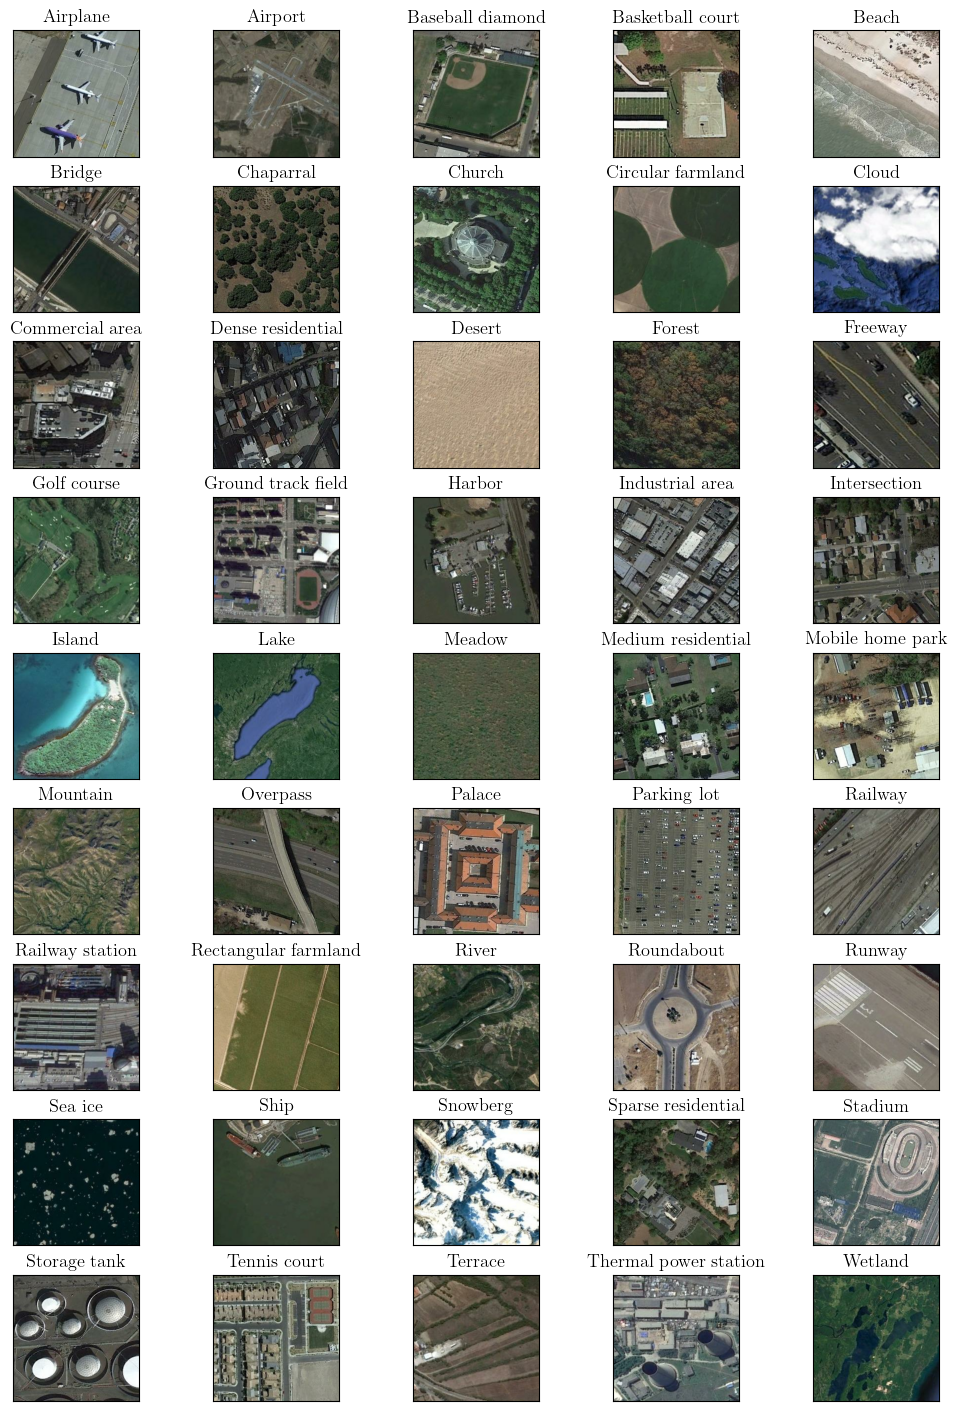
\includegraphics[width=\linewidth]{./assets/resisc45_all_classes.png}
    \caption{An example for each image class in the NWPU-RESISC45 dataset, taken from our test subset.}
\end{figure}
\end{appendices}

\section{Set5}
\begin{figure}[H]
    \centering
    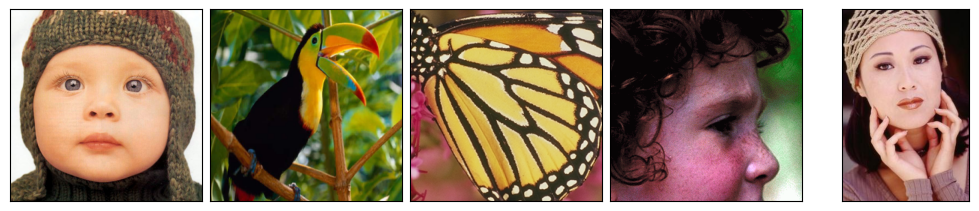
\includegraphics[width=\linewidth]{./assets/set5.png}
    \caption{The five images that make up the Set5 evaluation set.}\label{fig:model_comparison}
\end{figure}

\section{Set14}
\begin{figure}[H]
    \centering
    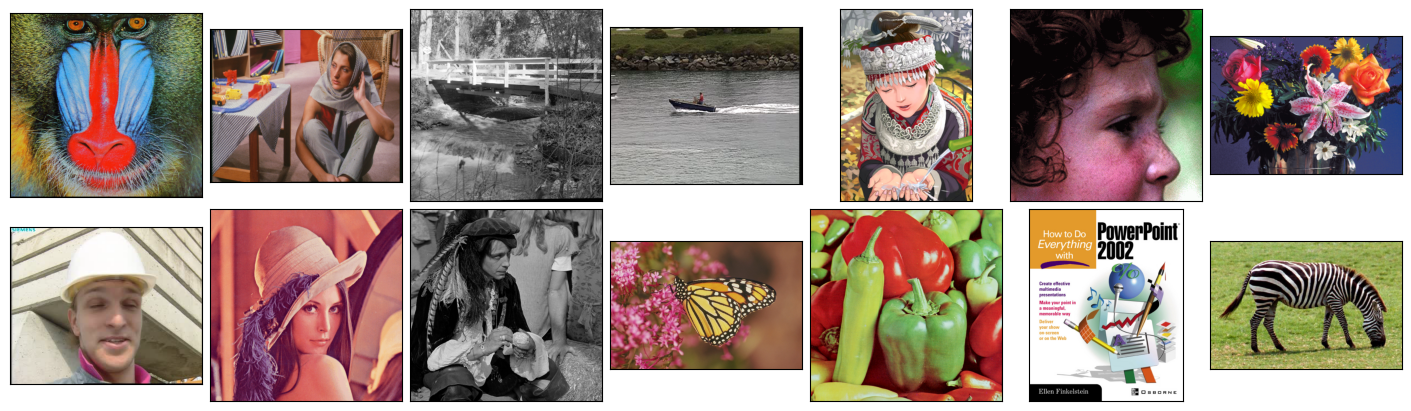
\includegraphics[width=\linewidth]{./assets/set14.png}
    \caption{The 14 images that make up the Set14 evaluation set.}\label{fig:model_comparison}
\end{figure}


